%\documentclass{neu_handout}
\documentclass[a4paper, 11pt]{article}

\usepackage{url}
\usepackage{amssymb}

\usepackage{url}
\usepackage{amssymb}
\usepackage{hyperref}
\usepackage{enumitem}
\usepackage{graphicx}
\usepackage{subcaption}
\usepackage{caption}

\usepackage{floatrow}


\usepackage{comment}  


\usepackage{comment}  
\usepackage{fullpage} % changes the margin
\usepackage[margin=1in]{geometry}
\pagenumbering{gobble}
\usepackage{hyperref}

\begin{document}


\title{DS5230 Update 2 : Pattern Recognition in Accidents in London}


\author{
  Sahasrabhojanee, Adwait\ \\     \texttt{sahasrabhojanee.a@husky.neu.edu}
  \and
  Sreekumar, Sreejith\  \\ \texttt{sreekumar.s@husky.neu.edu}
  \and
  Yu, Xue \\  \texttt{yu.xue1@husky.neu.edu}
  \and
  Li, Xuexian  \\ \texttt{li.xuex@husky.neu.edu}
}
\maketitle

\section{Introduction}

\subsection{Dataset}
The Department of Transport in the United Kingdom has extensively recorded road accidents over the years. For this project, we used data on road accidents occurring in the UK from 2009 to 2014, archived at Kaggle. The dataset has 33 columns, including the location (2 columns for postal co-ordinates, 2 columns for geographic co-ordinates) and the index of the accident. 

\subsection{Scope of the Project}

Our objective is to use unsupervised methods to extract patterns in road accidents, and recommend solutions to mitigate the number of accidents. \\ 

Although we were initially planning to conduct pattern recognition for the entire United Kingdom, after clustering on a few variables, we noticed that almost every clustering we made seemed to segregate the data into rural and urban areas. This is because of large difference in the values of the variables for accidents in rural areas and accidents in cities. Moreover, the vast majority of accidents in the dataset occurred in urban areas. Both of these seem to be a direct result of the population density of urban areas. \\ 

Consider Figure 1, which compares the geographic distribution of population density with the geographic distribution of the 'Accident Severity' variable in the dataset. It can be clearly seen that accidents having a severity of 1 tend to mostly happen in areas with high population density, while accidents assigned a severity of 3 tend to happen all over. The collection of red spots correspond to major cities, like London, Manchester, Liverpool, and Birmingham. \\ \\

\begin{figure}[H]
\begin{subfigure}[H]{0.4\linewidth}
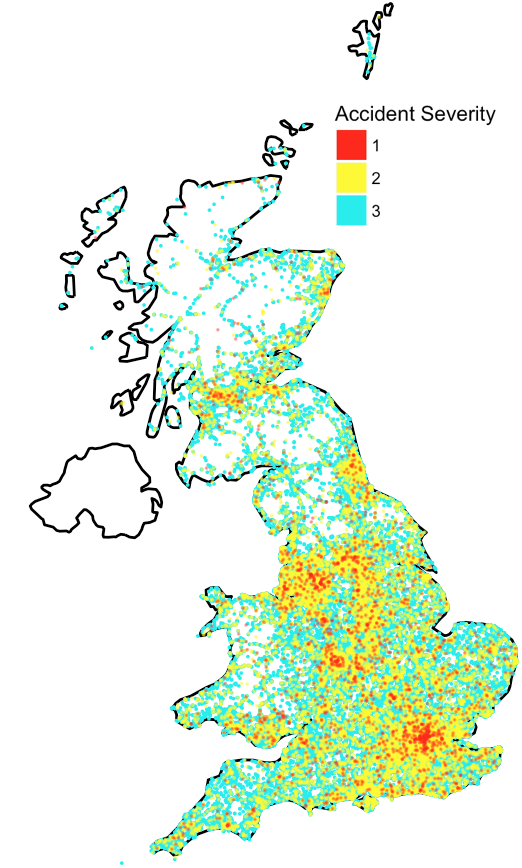
\includegraphics[height=9cm,keepaspectratio]{Severity_Map.png}
\caption{Accident Severity (2011)}
\end{subfigure}
\hfill
\begin{subfigure}[H]{0.4\linewidth}
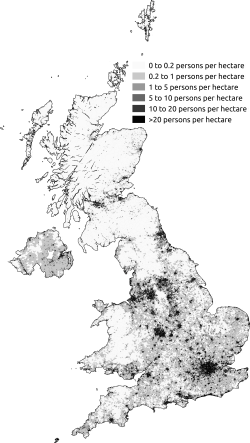
\includegraphics[height=9cm,keepaspectratio]{Population_density.png}
\caption{Population density (2011)}
\end{subfigure}%
\caption{Visible Similarity in Severity Patterns and Population Density}
\end{figure}

To form clusters other than the ones just splitting the accidents into those caused in cities and those caused outside cities, we have narrowed our focus to the Greater London area, which tops in the number of accidents continuously during all the six years under consideration. The data is explored further through standard exploratory data analysis,
principal component analysis and clustering techniques.

\section{Investigation of Traffic and Accidents in London}
\subsection{Patterns in road traffic}
We analyzed the annual average daily flow (AADF) of traffic in the roads of London to study the density of motor vehicles and isolate the busiest streets in London. Street in the UK are uniquely identified by an alpha-numeric numbering scheme[6]. This identifier appended to the Northing and Easting co-ordinates marks a unique fragment of the street in our analysis. \\ \\

Road fragments with similar characteristics in traffic were identified though cluster analysis.
\textit{K-means} was our candidate algorithm. Variables that quantify traffic of a region were manually selected, which included number of motor cycles, number of taxis, and the number bus coaches. The  experiment was performed with same parameters for every year between 2009 and 2014 to study the variations in areas with high traffic density. \textit{Silhouette method} was used to determine the optimal number of clusters, which was discovered to be two [Figure 7].\\ \\

Close examination of the clusters made it clear that the density of traffic in spots belonging to one of the clusters is very high compared to the ones in the second cluster. The co-ordinates of points belonging to this cluster was dropped on a map and it turns out they are very close to each other.\\ \\

\begin{figure}[H]
    \begin{center}
      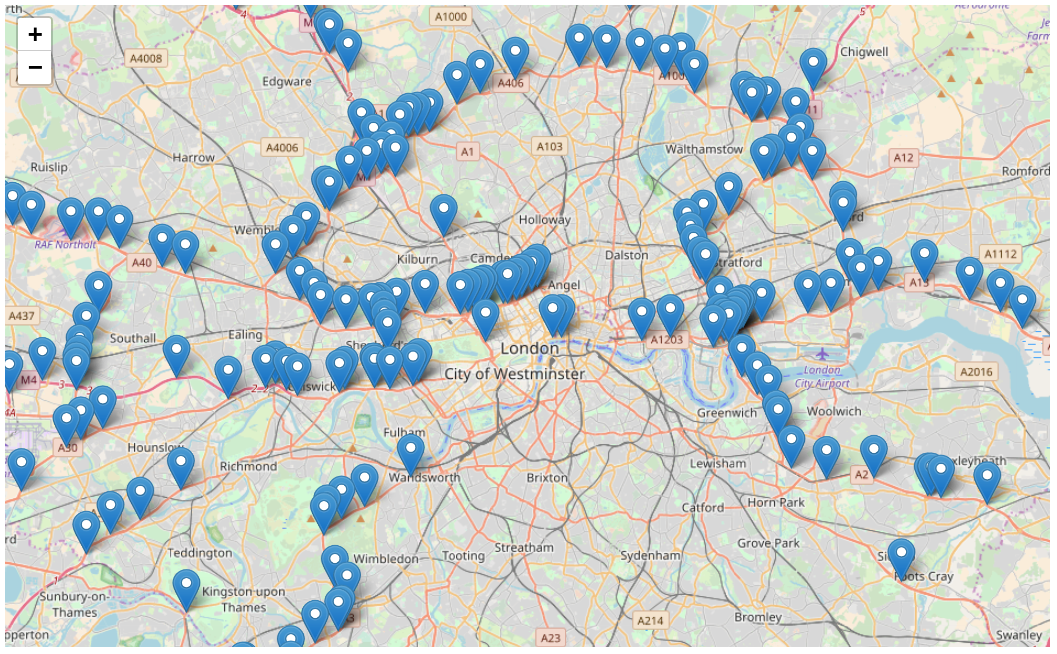
\includegraphics[height=9cm, width=20cm, keepaspectratio]{2009-hotspots.png}
      \caption{Hotspots for traffic flow in London (2009)}
    \end{center}
\end{figure}

In addition, we plotted yearly heatmaps of accidents to study how they correlate with the traffic flow plots. It can be observed that there is a positive correlation between the hotspots where traffic density is the highest and the number of accidents. In other words, high traffic flow zones in London are also accident prone areas. To illustrate this at one of the locations, consider the map segment which shows the traffic flow density on street A41 between Edgware Road(Circle District and Hammersmith \& City) and Baker Street[Figure 8,9]. This could be an indication that the traffic dense hotspots are not equipped enough to contain the traffic. A possible way of fixing this would be to build stack interchanges in this area.

\subsection{Segregation of Accidents in London using numeric attributes}

Our dataset had seven variables that were either ordinal or binary. We used \textit{k-means} and \textit{DBSCAN} to cluster on these variables, segregate accidents and then try to interpret the clusters. Our motivation for doing this was to look at a large cluster, try to figure out the causes of the accidents in the largest cluster and try to suggest a solution to reduce the accidents in the entire cluster. \\

We first applied Principal Component Analysis in the hope of reducing the time taken for DBSCAN to converge. \\ \\

\begin{figure}[H]
    \begin{center}
      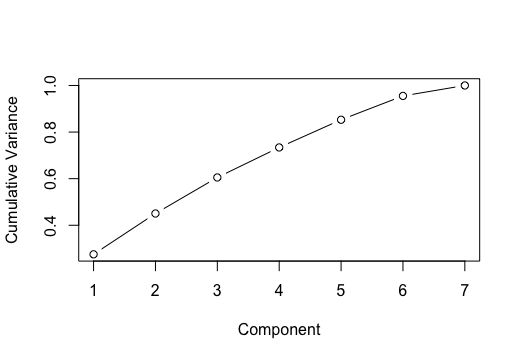
\includegraphics[height=9cm, width=20cm,keepaspectratio]{PCA.png}
      \caption{Cumulative Proportion of Variance Explained by Principal Components}
    \end{center}
\end{figure}

The first six components explained about 95\% of the variance. We thus managed to lower the number of dimensions by 1; not great, but better than nothing. \\ \\

We figured that two clusters would be relatively easy to interpret, and so we chose k = 2 for k-means, and adjusted the epsilon and MinPts of the DBSCAN clustering till we got two clusters. We used Forgy Initialization for k-means, with 20 initializations. Both the algorithms just segregated the accidents into two clusters depending on whether they were from Downtown London or the surrounding boroughs [Figure 13,14]. As there was no information in the dataset about what borough an accident occurred in, we were surprised, because we had not included the location of the accidents in the clustering. Upon further exploration, we discovered that one of the variables -- 'Police Force' -- was very high for accidents in Downtown London, and very low everywhere else. So we removed the Police Force variable, and tried clustering again, using K-means. The resulting cluster made no sense. We examined the data carefully and discovered that the data had a large number of observations, but not a large range of values that it's numeric variables could take. For example, Accident Severity could only take a value of 1, 2 or 3. We then decide to instead focus on some of the nominal variables.

\subsection{Road and Lighting conditions}

We discovered that the majority of accidents happen in the daylight, or when the street lights are present and lit in the darkness[Figure 5]. Further, looking over the conditions of the surface of the roads during the accidents, we see that a very large number of accidents occur on dry roads. Also, we noticed that around 20\% of the total number of accidents every year in Greater London happen when the roads are wet and damp. However, Greater London receives most of its rain during the months of Oct - Jan[4], and there is a chance that 20\% of accidents occur when the roads are wet because roads are wet 20\% of the time. Exploring the surface conditions in Greater London during different months, we found that accidents on wet roads are present throughout the year.\\ \\

We clustered the accidents based on Road Surface Conditions, Carriageway Hazards, Special Conditions at Site, and Light Conditions, which were all nominal variables. We used the \textit{Dice co-efficient} as a distance metric for these columns, and then clustered them using the \textit{k-medoids algorithm}. K-medoids works much the same way as k-means, but with a couple of differences. Unlike k-means, k-medoids always selects data points as the centers, for every iteration. This makes it a viable option for nominal data, as clustering around a point that does not exist in the dataset only makes sense for continuous or ordinal variables. Also, k-medoids uses the Manhattan Distance, and not the Euclidean Distance, as is common in k-means [6]. The silhouette was computed for k = 2 to 10, and a k of 4 was chosen [Figure 10], having a silhouette of 0.95. \\ \\

After visualizing a few data points from each cluster, it can be seen that the Light Conditions and Road Surface Conditions variables have been given importance by the clustering algorithm, and the four clusters are four combinations of these two variables [Figure 11]. Below are the accidents belonging to each cluster plotted on maps. \\ \\

\begin{figure}[H]
    \begin{center}
      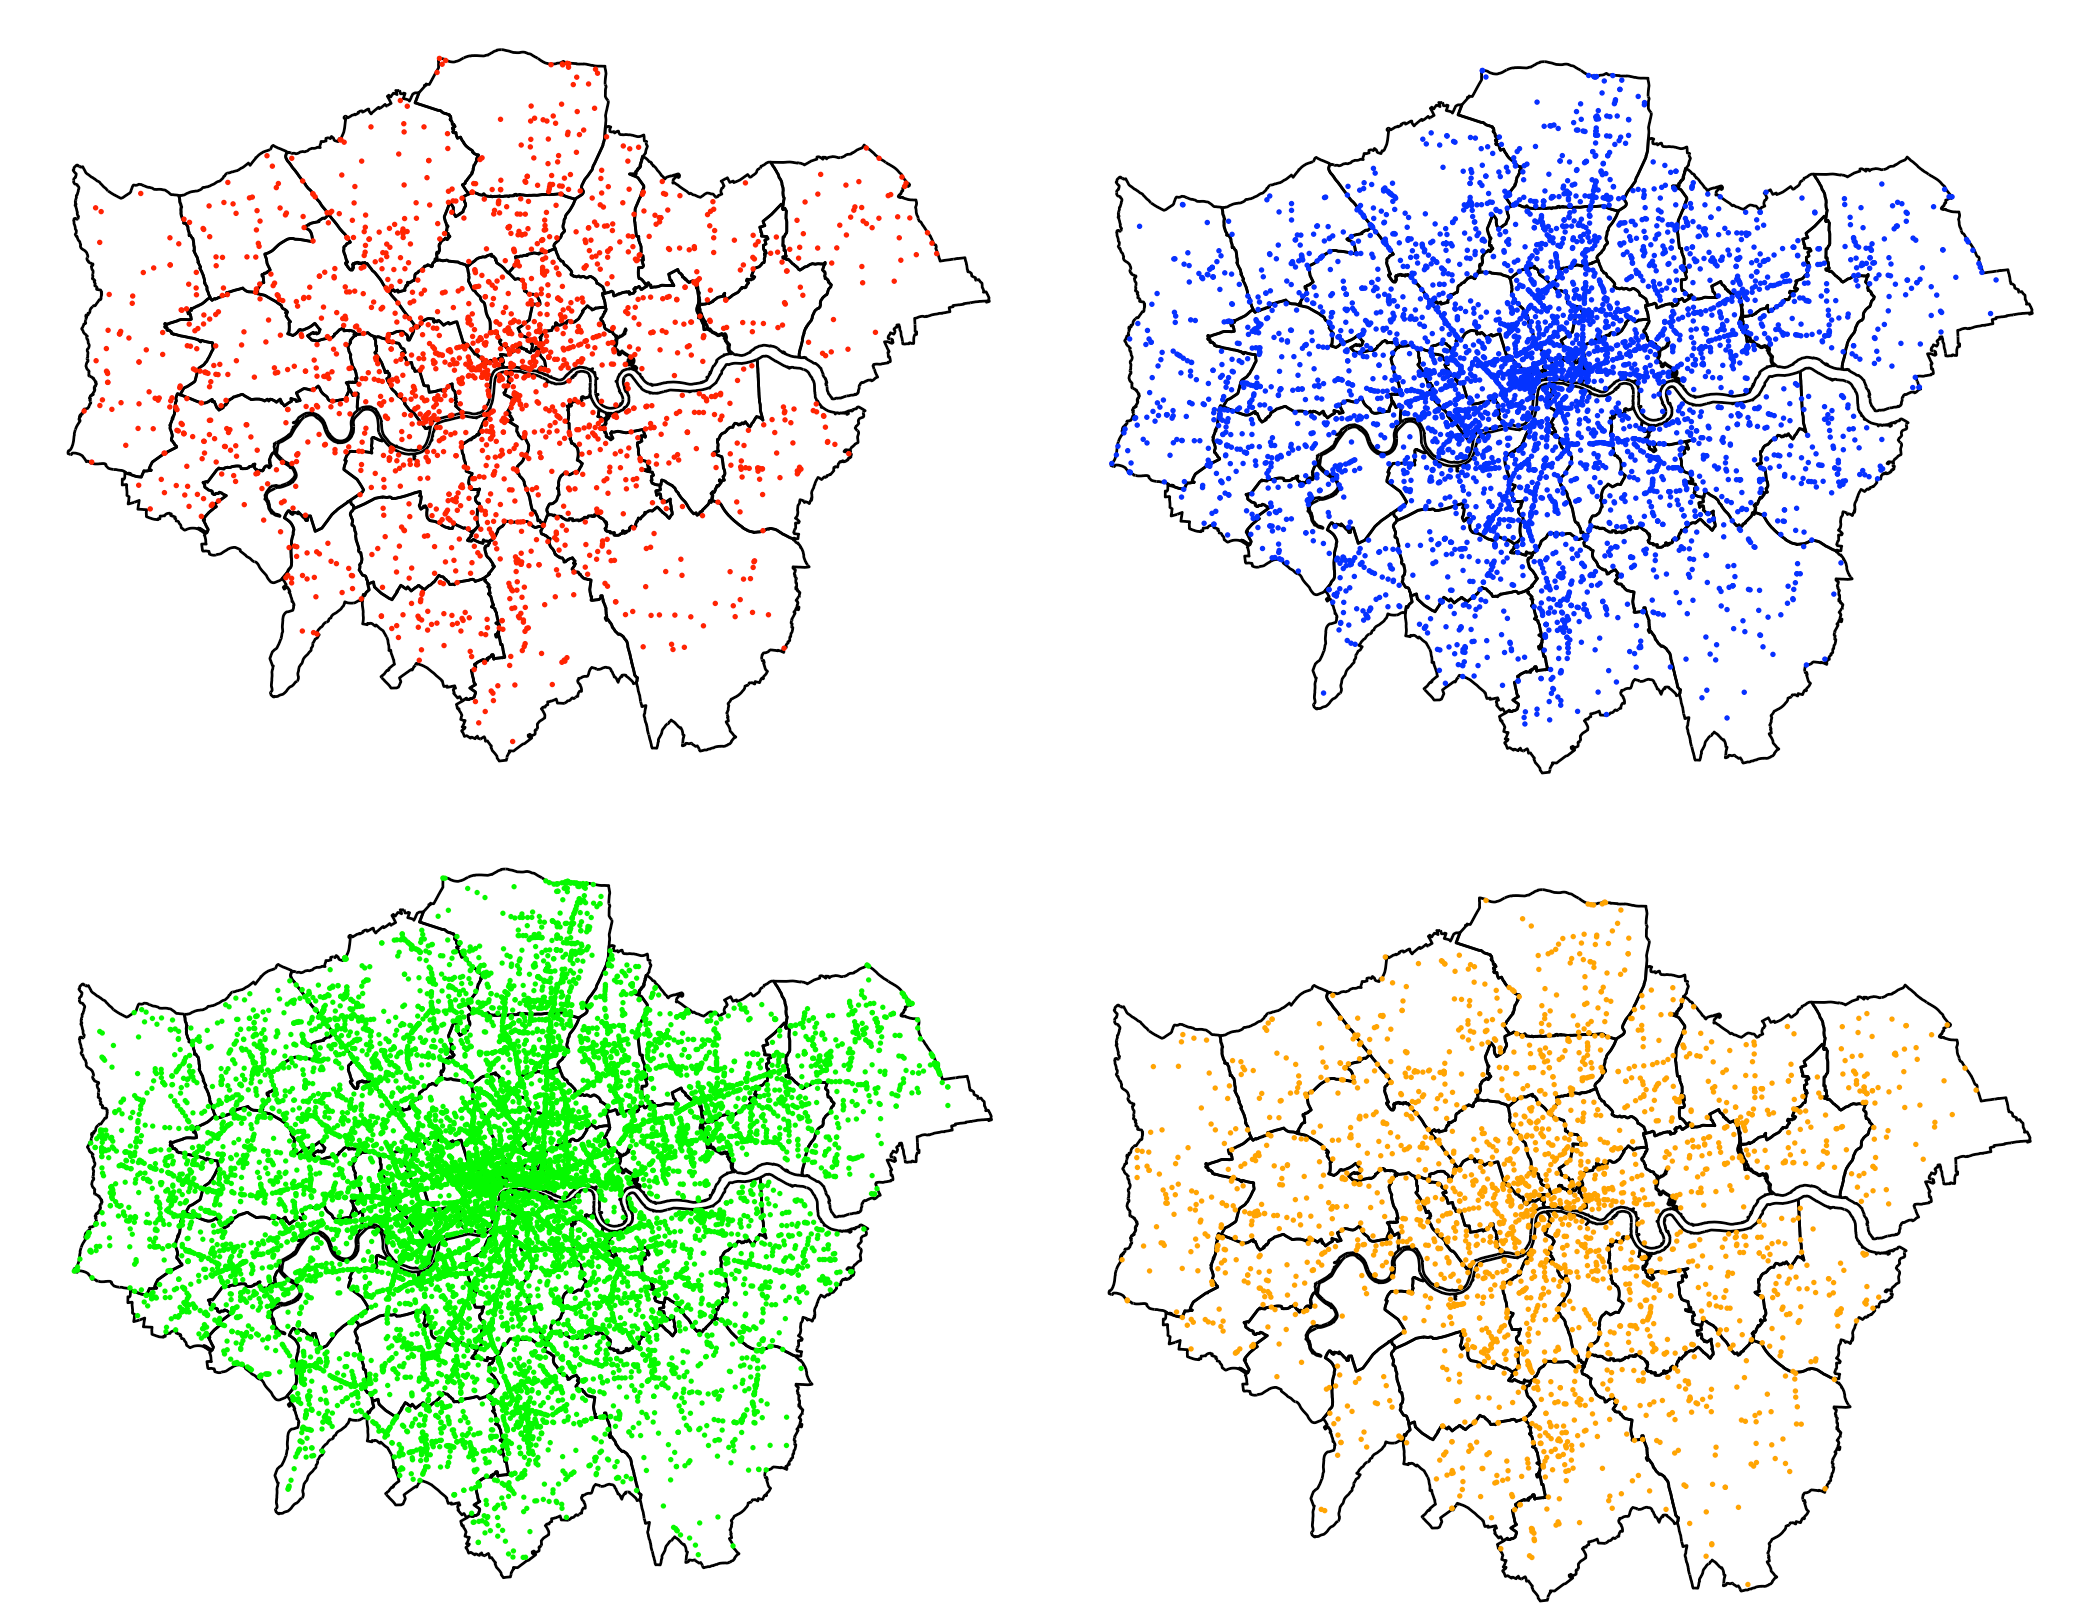
\includegraphics[height=9cm, scale=0.01,keepaspectratio]{4_clusters.png}
      \caption{Clustering for Road and Lighting conditions}
    \end{center}
\end{figure}

The plots of the four clusters show that two of the clusters (red and orange) contain a much higher \textit{proportion} of accidents that occurred away from Downtown London than the other two clusters.
As can be seen in Figure 11, the common important variable between these clusters is the road surface condition. It would seem from this clustering that a Wet/Damp road has a higher chance of causing an accident as you move away the heart of the city. \\ \\

A possible explanation for this is the increase in speed limit as you head out of downtown London [Figure 12]. People going faster on wet roads would have a higher chance of losing control of their car. The accidents caused outside of Downtown London might be reduced if the speed limit was lowered in rainy months.

\section{Next Steps}

We will try to see whether our findings for London also hold true for other major cities/urban areas in the UK. 
\pagebreak
\section{Appendix}

\begin{figure}[H]
    \begin{center}
      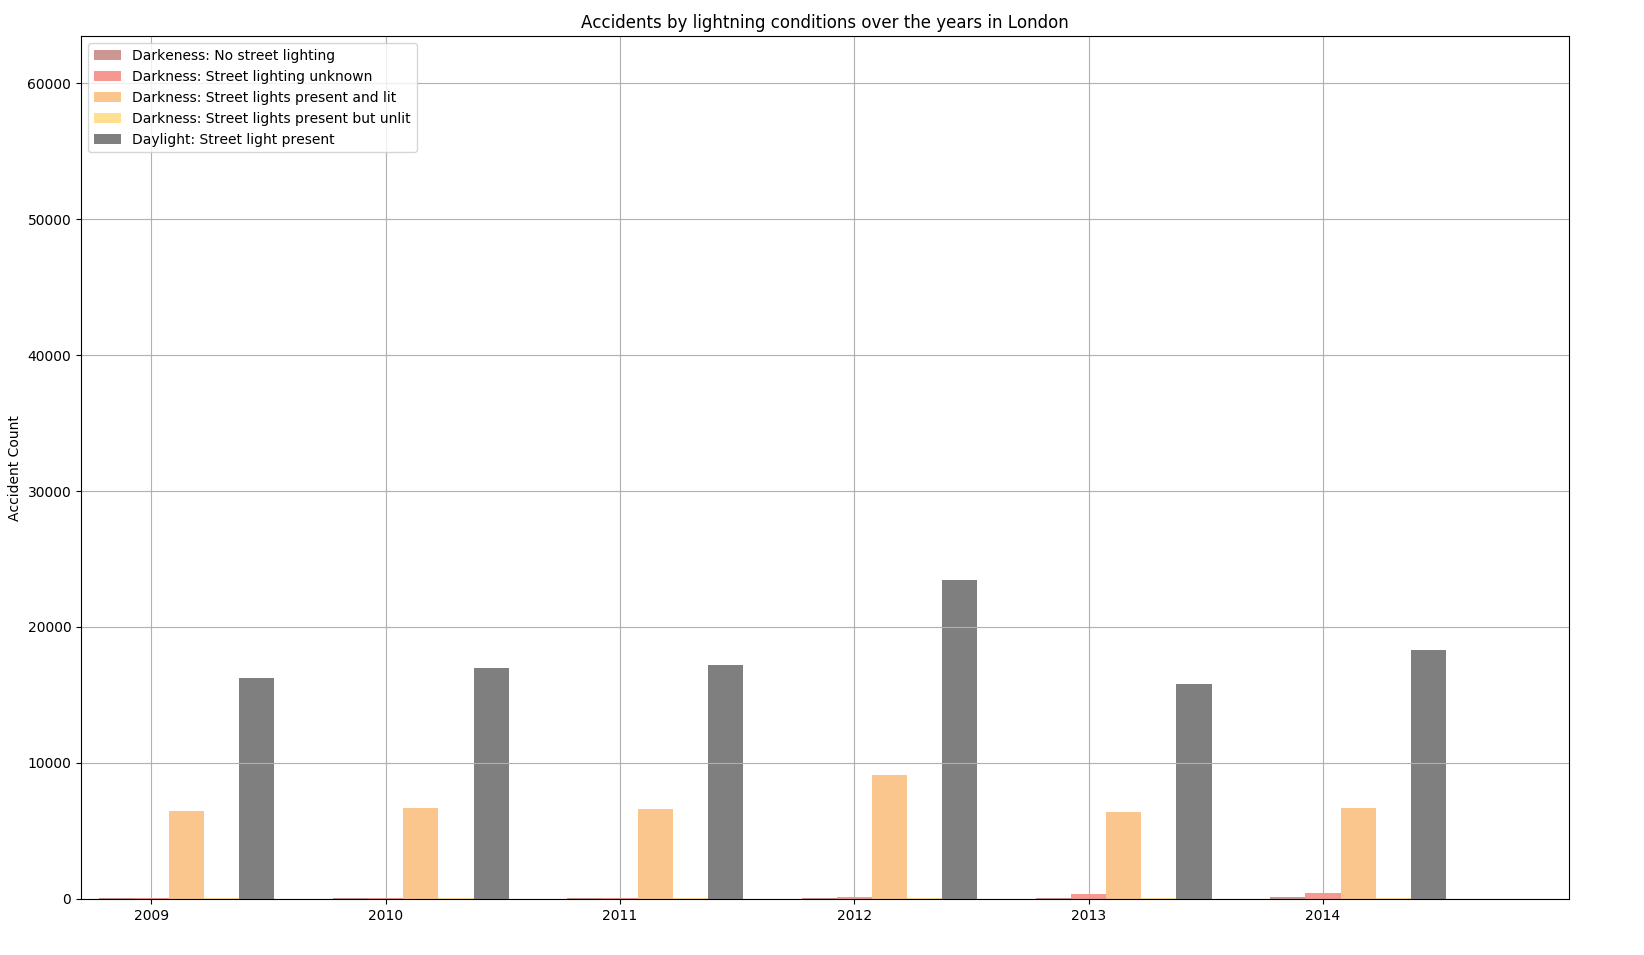
\includegraphics[height=9cm, width=20cm,keepaspectratio]{light-conditions-london.png}
      \caption{Frequency of accidents with lighting conditions at the time of accidents in London}
    \end{center}
\end{figure}

\begin{figure}[H]
    \begin{center}
      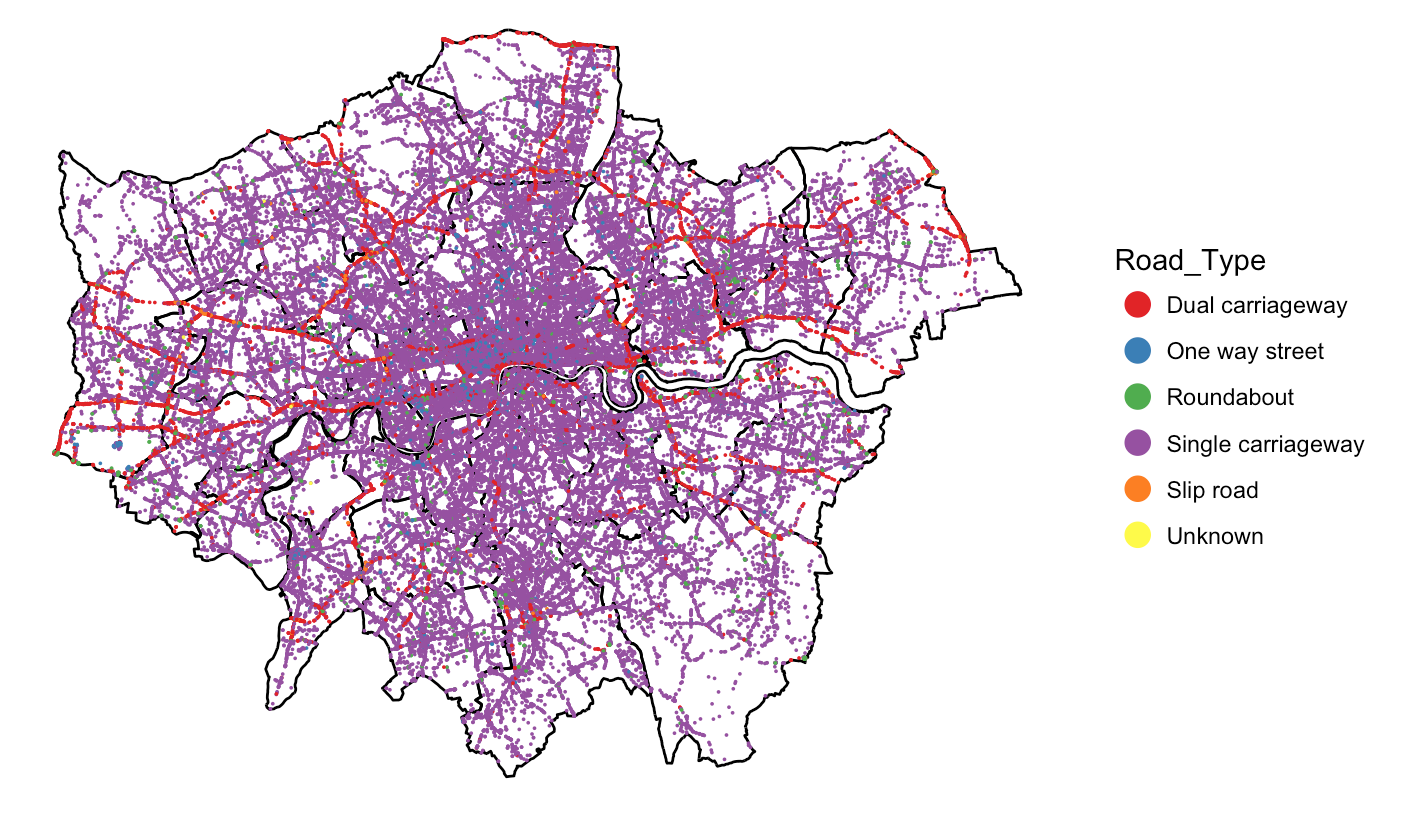
\includegraphics[height=9cm, scale=0.01,keepaspectratio]{london_roads.png}
      \caption{Road Types in London}
    \end{center}
\end{figure}

\begin{figure}[H]
    \begin{center}
      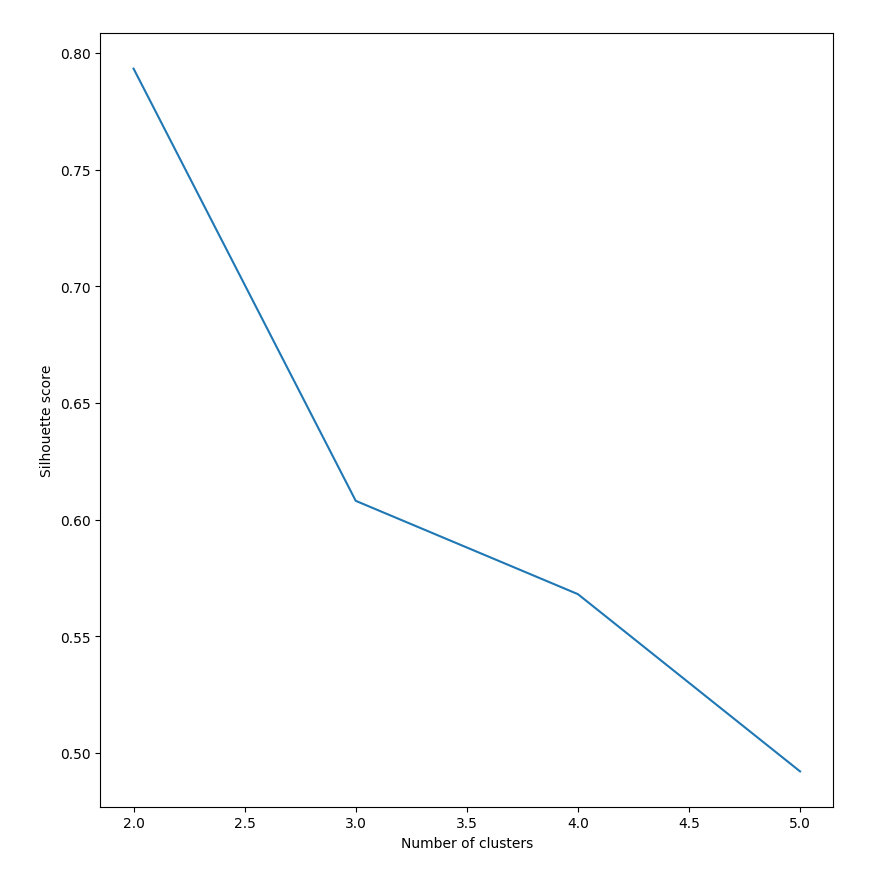
\includegraphics[height=4.5cm, scale=0.01,keepaspectratio]{silhouette-score-traffic.png}
      \caption{Silhouette Plot for Road Traffic Cluster Analysis}
    \end{center}
\end{figure}

\begin{figure}[H]
    \begin{center}
      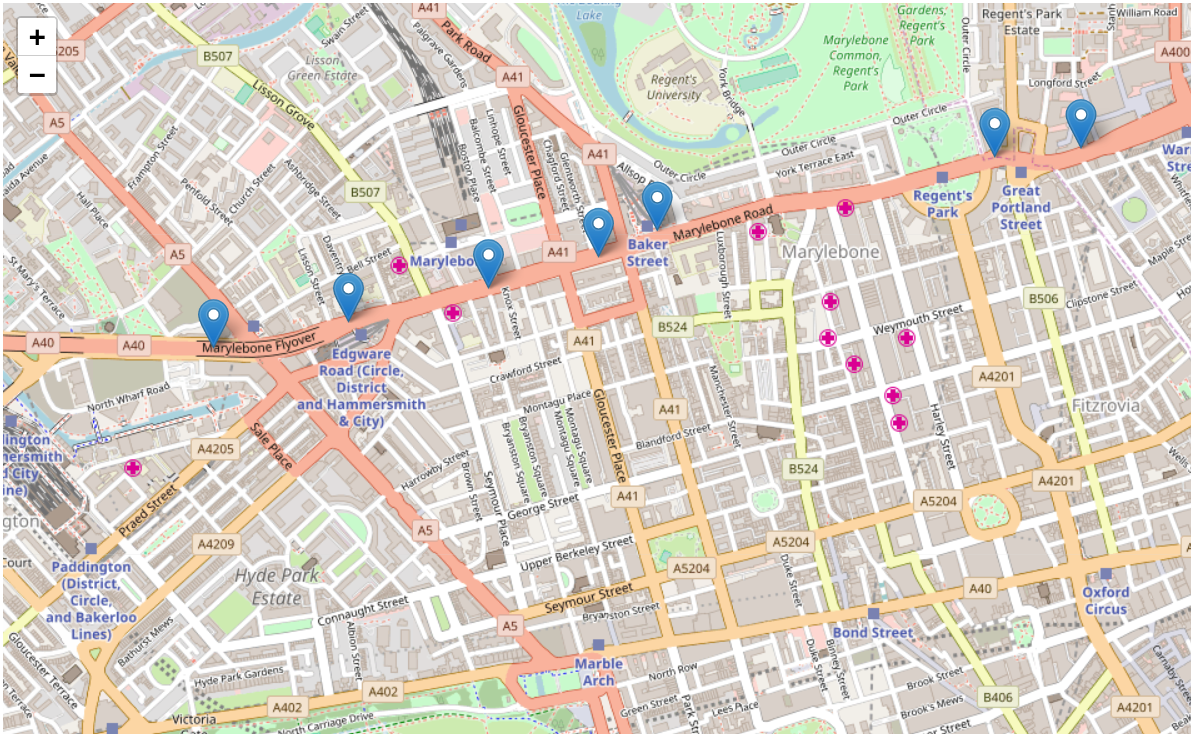
\includegraphics[height=9cm, width=20cm,keepaspectratio]{traffic-bakers-street.png}
      \caption{High density traffic region Baker's street and Edgware Road}
    \end{center}
\end{figure}

\begin{figure}[H]
    \begin{center}
      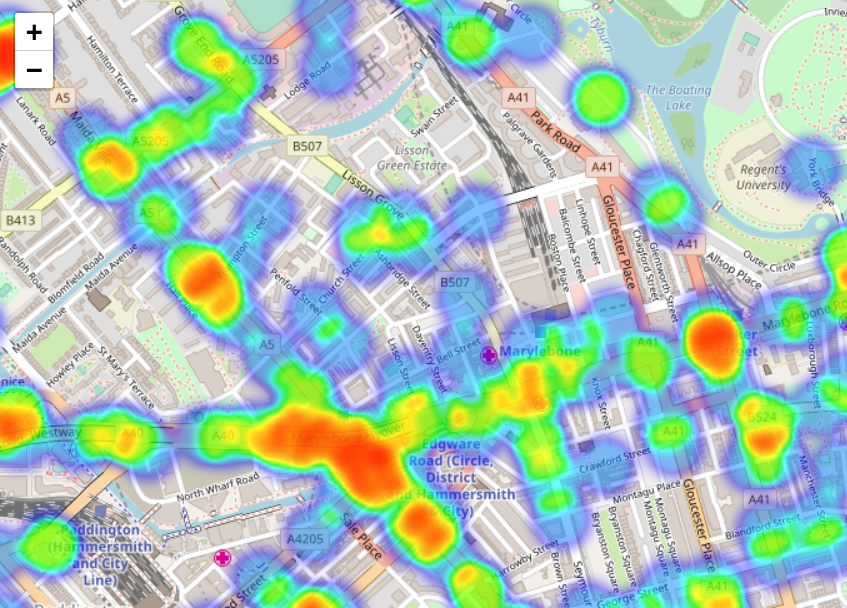
\includegraphics[height=9cm, width=25cm,keepaspectratio]{accident-2009-heatmap-bakers-street.png}
      \caption{Heatmap of Accidents around Baker's street and Edgware Road}
    \end{center}
\end{figure}

\begin{figure}[H]
    \begin{center}
      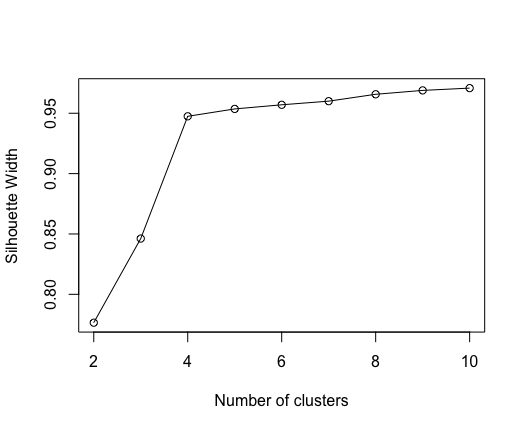
\includegraphics[height=4.5cm, scale=0.4,keepaspectratio]{silhouette_road_conditions.png}
      \caption{Silhouette Plot for Road and Lighting conditions}
    \end{center}
\end{figure}


\begin{figure}[H]
    \begin{center}
      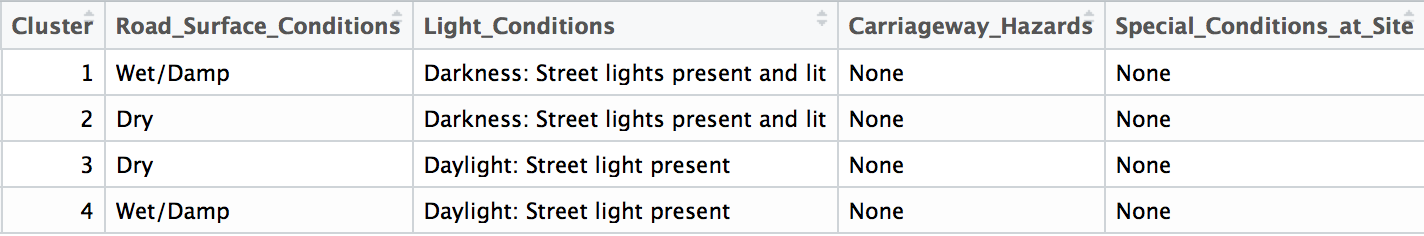
\includegraphics[height=2.5cm,keepaspectratio]{cluster_eg.png}
      \caption{Examples of Clustered Datapoints for Road and Lighting conditions}
    \end{center}
\end{figure}

\begin{figure}[H]
    \begin{center}
      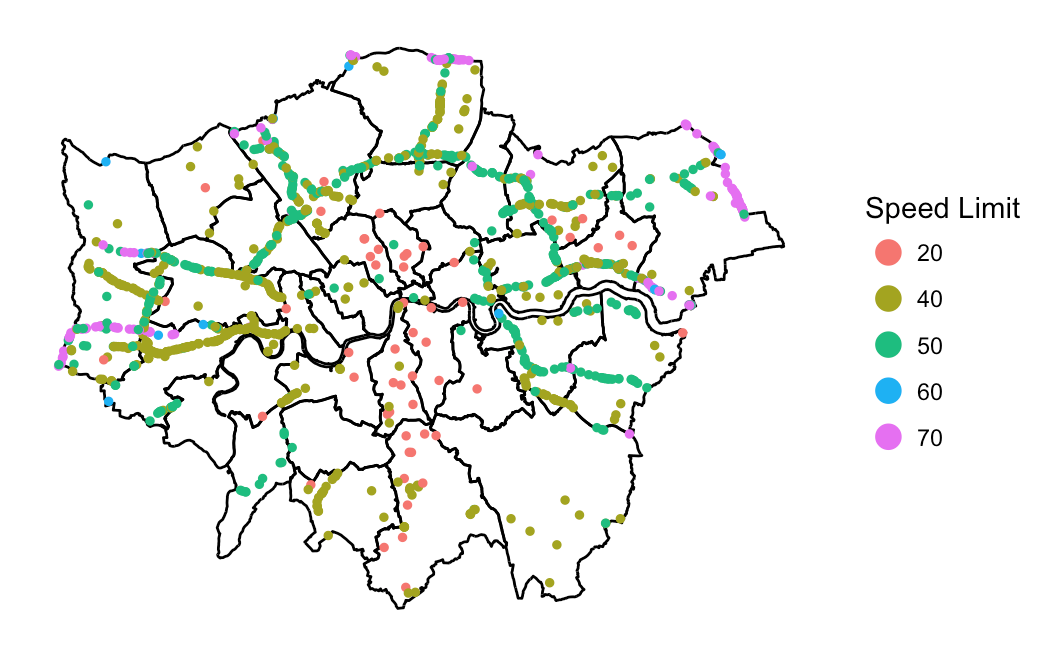
\includegraphics[height=7cm,keepaspectratio]{sl_london.png}
      \caption{Accidents by Speed Limit (Excluding the Ubiquitous Speed Limit of 30)}
    \end{center}
\end{figure}

\begin{figure}[H]
    \begin{center}
      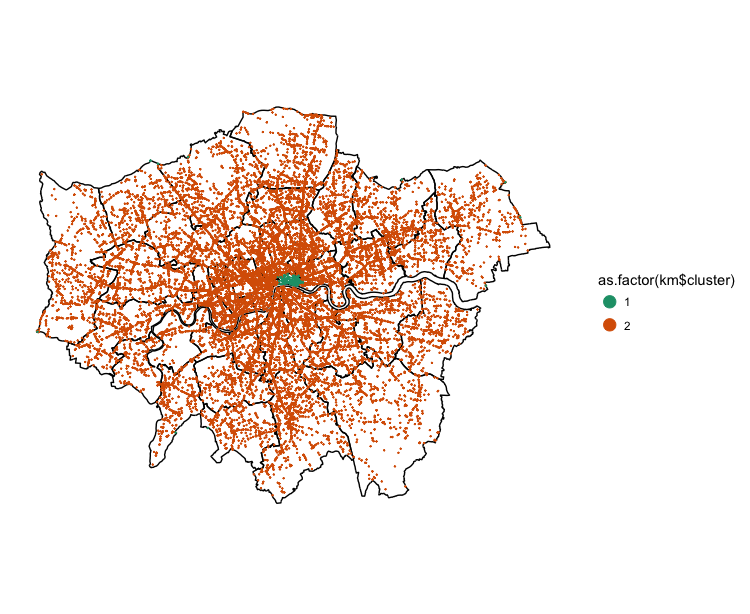
\includegraphics[height=9cm,keepaspectratio]{km_1_county.png}
      \caption{K-means Clustering on Numeric Columns Separates One Borough from the Others}
    \end{center}
\end{figure}

\begin{figure}[H]
    \begin{center}
      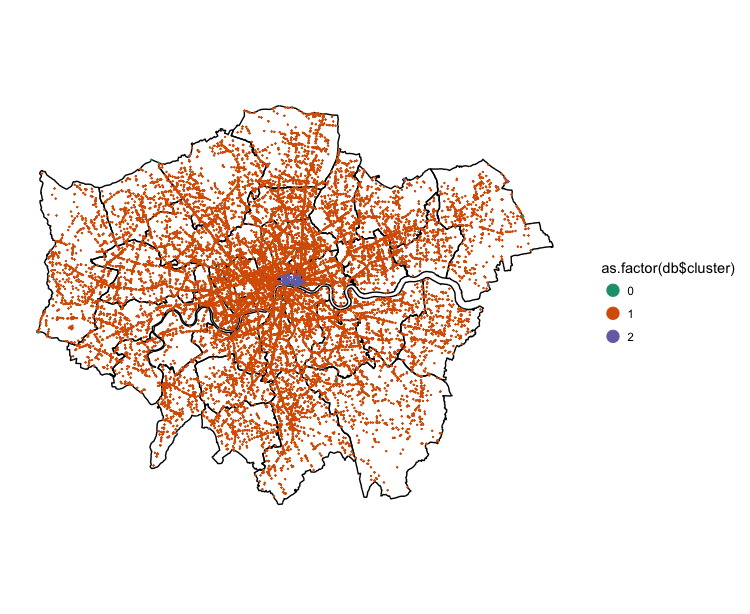
\includegraphics[height=9cm,keepaspectratio]{db_1_county.png}
      \caption{DBSCAN Clustering on Numeric Columns Separates One Borough from the Others (Cluster 0 indicates Outliers)}
    \end{center}
\end{figure}


\section{References}
 [1] \href{https://data.london.gov.uk/dataset/statistical-gis-boundary-files-london}{London Shapefile}
 \newline
 [2] \href{http://www.naturalearthdata.com} {UK Shapefile}
 \newline
 [3] \href{https://en.wikipedia.org/wiki/Demography_of_the_United_Kingdom}{Demography of the United Kingdom}
 \newline
 [4] \href{http://projectbritain.com/climate.html}{London Yearly Rainfall Distribution}
 \newline
 [5] \href{https://en.wikipedia.org/wiki/Great_Britain_road_numbering_scheme}{Great Britain road numbering scheme}
 \newline
 [6] \href{https://en.wikipedia.org/wiki/K-medoids}{k-medoids}
 \newline

\end{document}

%%% Local Variables:
%%% mode: latex
%%% TeX-master: t
%%% End:




